\documentclass[12pt]{article}
\usepackage[utf8]{inputenc}
\usepackage[spanish, es-tabla]{babel}
\usepackage{graphicx}
\usepackage{float}


\title{Segmentación 3D de manchas de sustancia blanca (WML)}
\date{19/05/2019}
\author{J. Gamazo, G. Izaguirre, G. Cabrera \\
	 Universidad Nacional de Educación a Distancia}


\begin{document}
	\pagenumbering{gobble}
	\maketitle
	\newpage
	\paragraph{}
	\newpage
	\pagenumbering{arabic}
	\tableofcontents
	\newpage
	
	\renewcommand{\abstractname}{Resumen}

	\begin{abstract}
	Este es el resumen.
	\end{abstract}
	
	
	\renewcommand{\abstractname}{\textit{Abstract}}
	
	\begin{abstract}
	This is the abstract.
	\end{abstract}

	\newpage
	
	\section{Introducción}

	\paragraph{}
	En 2017, en las conferencias MICCAI (\textit{Medical Image Computing and Computer Assisted Intervention}), fue lanzado el concurso de Segmentación de Hiperintensidades de materia blanca. Este se trata de un concurso de análisis de imágenes médicas, en el que se pretende comparar directamente métodos para la segmentación automática de Hiperintensidades de Materia Blanca en el cerebro.

	\paragraph{}
	El interés en este campo radica en que estas hiperintensidades se encuentran comúnmente en personas mayores y están asociadas con varios desórdenes neurológicos y geriátricos, como problemas de humor o deterioro cognitivo.

	\paragraph{}
	Normalmente son encontradas en magneto-resonancias FLAIR y, aunque es posible marcar las zonas donde se encuentran las hiperintensidades a mano, es una tarea bastante laboriosa. Es por ello que técnicas basadas en la visión artificial y en aprendizaje máquina han ganado mucho peso en los últimos año, como una forma bastante prometedora para el diagnóstico automático de enfermedades.

	\paragraph{}
	En cuanto al concurso, desde la propia organización se proporciona un conjunto de entrenamiento que todos los participantes deben descargar y usarlo para desarrollar su propio método, el cual debe ser contenedorizado con Dockers. El conjunto de test es guardado por la organización y no es hecho público en ningún momento, siendo únicamente utilizado para evaluar los distintos métodos. Para esta evaluación, además,  se han utlizado cinco métricas: coeficiente de similaridad de Dice, distancia de Hausdorff, diferencia absoluta de volumen, sensitividad para lesiones individuales y puntuación F1 para lesiones individuales.
	
	\paragraph{}
	En este artículo se presentan los cambios realizados en uno de estos modelos, en concreto el ganador, el cual hace uso de una variante de redes totalmente convolucionales basada en U-Net. Estos cambios han sido la creación de una GAN para conseguir un aumento significativo en el volumen de datos de entrenamiento.
	
	\subsection{Estado del arte}

	\paragraph{}
	El método base a utilizar, descrito más en detalle en el artículo de Hongwei Li et al. \cite{Fully convolutional network ensembles for white matter hyperintensities segmentation in MR images}, ha sido el ganador de este concurso, y se basa en el uso de una variante de redes convolucionales basada en U-Net.
	
	\paragraph{}
	Así, su arquitectura toma como entrada los cortes axiales de dos modalidades de escáneres MR, T1 y FLAIR, las cuales son juntadas como entrada de dos canales. En la imagen inferior se puede observar dicha arquitectura.
	
	\paragraph{}
	
	\begin{figure}[h!]
	\centering
		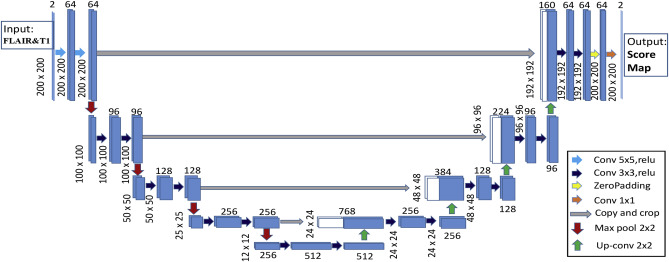
\includegraphics[width=\linewidth]{img1.jpg}
		\caption[\textit{Arquitectura del modelo}]{Arquitectura del modelo}
		\label{fig:FCC}
	\end{figure}

	\paragraph{}
	En este modelo, dos capas convolucionales son usadas de forma repetida, cada una seguida por una unidad de rectificado lineal (ReLU) y una operación max-pooling de 2 x 2 con paso 2. En la capa final, una convolución de 1 x 1 es utilizada para mapear cada vector de características de 64 componentes en dos clases. En total, se utilizan 19 capas convolucionales. 
	
	\paragraph{}
	Como función de pérdida se utiliza la pérdida de Dice, la cual es formulada de la siguiente forma:
	
	\begin{figure}[H]
	 	\centering
		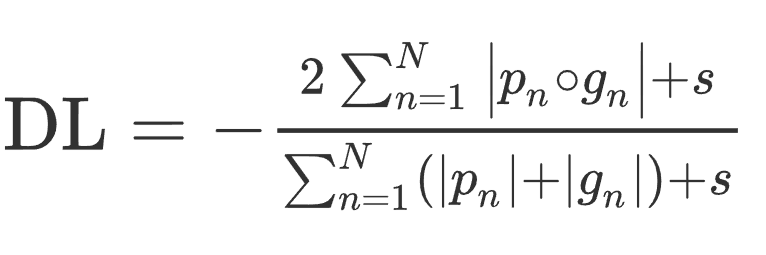
\includegraphics[height=2cm]{dice_loss.png}
		\label{fig:Dice}
	\end{figure}
	
	\paragraph{}
	donde G=\{g$_{1}$, .... g$_{N}$\} es la probabilidad observable de segmentación sobre N capas, y P=\{p$_{1}$, ..., p$_{N}'$\} la probabilidad predicha sobre N capas.
	
	\paragraph{}
	Por último, cabe mencionar que este método, como su nombre indica, utiliza técnicas de conjuntos, las cuales son útiles para reducir los problemas de exceso asociados a las redes neuronales. Estas combinan múltiples modelos de aprendizaje para obtener mejor rendimiento a la hora de predecir.
	
	\newpage
	
	\section{GAN: Generative Adversial Networks}
	
	\newpage
	
	\section{Implementación}
	
	\newpage
	
	\section{Resultados}
	
	\newpage
	
	\section{Conclusiones}
	
	\newpage
	
	\begin{thebibliography}{9}
	\raggedright
	
	\bibitem{Fully convolutional network ensembles for white matter hyperintensities segmentation in MR images}
	H. Li, G. Jiang, J. Zhang, R. Wang, Z. Wang, W. Zheng y B. Menze. \textit{Fully convolutional network ensembles for white matter hyperintensities segmentation in MR images}, 2018
	
	\bibitem{Data Augmentation in Deep Learning}
	T. Neff. \textit{Data augmentation in deep learning using generative adversial networks}, 2018

	\end{thebibliography}
	
\end{document}